\documentclass[12pt]{report}
\usepackage{graphicx}
\usepackage{amsmath}
\usepackage{tocbibind} % To include the bibliography in the table of contents
\usepackage{setspace} % For line spacing
\usepackage{url} 
\usepackage{hyperref}
\usepackage{graphicx}
\usepackage{caption}
\usepackage{float}
\usepackage{subcaption}
\usepackage{amsmath}
\usepackage{listings}
\usepackage{xcolor}
\usepackage[linesnumbered,ruled,vlined]{algorithm2e}
\usepackage{mhchem}

\newcommand{\var}[1]{\textcolor{blue}{\texttt{#1}}} % Command for variables
\newcommand{\kw}[1]{\textcolor{purple}{\texttt{#1}}} % Command for keywords


\setlength{\parindent}{0pt}


\begin{document}

% Title page
\begin{titlepage}
    \centering
    %\vspace*{2cm} % Optional vertical space at the top

    {\Huge \textbf{Prediction of Ignition Delay Time Characteristics of Natural Gas Mixture Using Machine Learning Models}\par}
    \vspace{1cm} % Optional space between sections
    
    {\Large B.Tech. project report submitted in partial fulfillment of the requirements for the award of}\par
    
    {\Large Bachelor of Technology in Energy Engineering}\par
    
    \vspace{1cm}
    
    \textbf{by}\par
    {\Large Rushil Mital}\par
    \vspace{0.5cm}
    {\Large 2021ES10184}\par
    
    \vspace{0.5cm} % Optional space for separation
    
    \textbf{Under the Guidance of}\par
    {\Large Prof Snehasish Panigrahy}\par
    
    \vspace{0.5cm} % Optional space for separation

    % Include the logo image
    \begin{figure}[H]
        \centering
        \includegraphics[width=0.3\textwidth]{institute_logo.png} % Adjust the width as necessary
    \end{figure}
    
    {\Large Department of Energy Science and Engineering}\par
    \vspace{0.25cm}
    {\Large INDIAN INSTITUTE OF TECHNOLOGY DELHI}\par
    \vspace{0.25cm}
    {\Large NEW DELHI – 110016}\par
    {\Large November 2024}\par

\end{titlepage}


\newpage

% Appendix B
\section*{ \centering Undertaking by the Student}
I hereby declare that the work presented here in the report/thesis has been carried out by me towards the partial fulfilment of the requirement for the award of Bachelor of Technology in Energy Engineering at the Department of Energy Science and Engineering, Indian Institute of Technology Delhi. The content of this report in full or in parts has not been submitted to any other institute or university for the award of any degree.
\vspace{2cm}


Rushil Mital \hfill 2021ES10184 \\
8095223457 \hfill Rushil.Mital.es121@dese.iitd.ac.in \\
Place: Delhi \hfill Date: 25th November 2024

\newpage

% Appendix C
\section*{\centering Certificate by the Supervisor}
This is to certify that the report/thesis entitled “Prediction of Ignition Delay Time Characteristics of Natural Gas Mixture Using Machine Learning Models” being submitted by Rushil Mital (2021ES10184) to the Department of Energy Science and Engineering, Indian Institute of Technology Delhi, for partial fulfilment of the requirement for the award of the degree of Bachelor of Technology in Energy Engineering. This study was carried out by him under my guidance and supervision.

\vspace{1cm}

\begin{flushright}
Signature of the supervisor: \\
Prof Snehasish Panigrahy \\
Department of Energy Science and Engineering \\
Indian Institute of Technology Delhi
\end{flushright}

Place: New Delhi \\
Date: 25th November 2024\\



\newpage
\section*{\centering Acknowledgements}
I would like to express my sincere gratitude to Professor Snehasish Panigrahy for his invaluable guidance and support throughout this project. I am also thankful to the Department of Energy Science and Engineering at IIT Delhi for providing me with the opportunity and resources to undertake this research. Their support has been instrumental in the successful completion of this work.

\vspace{1cm}
\begin{flushright}
Rushil Mital
\end{flushright}
\newpage
\section*{\centering Abstract}
% Content goes here
Hydrogen-compatible gas turbines present a viable solution for decarbonizing electricity generation. However, the combustion and handling of hydrogen are non-trivial due to its high reactivity and propensity to detonate. Critical safety parameters, such as auto-ignition delay times, can be predicted using detailed kinetic models. However, the computational expense of such models poses a challenge for their integration with fluid dynamics simulations. To address this, an auto-ignition prediction tool was developed based on an artificial intelligence (AI) model, allowing for rapid computations and its integration into an explosion model. 

A dataset of ignition delay times (IDTs) was generated automatically using a recently developed detailed kinetic model from the National University of Galway (NUIG), as reported in the literature. The generated dataset spans a broad operational range, accounting for various fuel compositions. To mitigate clustering in the sample points, a quasi-random Sobol sequence was employed, ensuring uniform coverage of the input parameter space. Multiple algorithms were trained, cross-validated, and tested using a database of over 70,000 ignition cases involving natural gas/hydrogen blends. The training and testing datasets were divided in a standard 70/30 split. The AI model demonstrated significant robustness, achieving an average correlation coefficient of over 99.91\% for both the training and testing datasets, with a mean absolute error (MAE) of approximately 0.03 and a mean squared error (MSE) below 0.04. Furthermore, tests confirmed the model's robustness beyond the pressure, temperature, and equivalence ratio ranges found in the dataset.




% Table of Contents
\tableofcontents
% List of Figures
\listoffigures


\section*{Nomenclature/Abbreviations}
\begin{tabbing}
    IDT \hspace{1cm} \= Ignition Delay Time \\
    ANN \> Artificial Neural Network\\
    KNN \> K Nearest Neighbours\\
    MLP \> Multilayer Perceptron
\end{tabbing}


\newpage

% Chapter Structure (Template)

\chapter{Literature Review}
The combustion characteristics of hydrogen, syngas, and hydrocarbon-based fuels have garnered significant attention in recent years, driven by the need to reduce carbon emissions and optimize energy production in power generation systems. As hydrogen and syngas emerge as viable alternatives to traditional fossil fuels, understanding their combustion properties—such as ignition delay times, flame speeds, and the influence of different fuel blends—becomes crucial for the safe and efficient operation of internal combustion engines and gas turbines. However, the high reactivity of these fuels, especially hydrogen, presents unique challenges that necessitate the development of advanced predictive models.

Recent research efforts have focused on experimental studies, detailed chemical kinetic modeling, and the integration of machine learning (ML) and artificial intelligence (AI) techniques to better predict combustion behaviors under a wide range of operating conditions. The following literature review synthesizes findings from studies that explore hydrogen and syngas oxidation, C1-C2 hydrocarbons combustion, and the development of AI-driven models for predicting auto-ignition delay times.


\section{Combustion and Flame}

\subsection{Introduction}
The transition to cleaner energy sources has driven significant research into hydrogen (H$_2$) and syngas (H$_2$ and CO mixtures) as potential fuels. These fuels have garnered attention for their ability to reduce greenhouse gas emissions when compared to conventional carbon-based fuels. Syngas, in particular, can be derived from biomass gasification, making it a sustainable option for energy production. This review outlines key studies on the combustion characteristics, chemical kinetics, and applications of hydrogen and syngas, focusing on high-pressure and high-temperature conditions.

\subsection{Hydrogen as a Combustion Fuel}
Hydrogen has been widely studied due to its potential to be a clean fuel with low emissions, primarily producing water vapor during combustion. Early work, such as by Lee and Hochgreb (1998) and Mittal et al. (2006), focused on understanding the combustion behavior of hydrogen under controlled conditions, such as rapid compression machines (RCMs) and shock tubes, to assess ignition delay times and flame speeds. These studies showed that hydrogen exhibits high reactivity, with ignition delay times decreasing as pressure and temperature increase.

In terms of chemical kinetics, hydrogen combustion is largely governed by reactions involving hydroxyl (OH) and hydroperoxyl (HO$_2$) radicals. Reactions such as 
\begin{equation}
\text{H} + \text{O}_2 \rightarrow \text{OH} + \text{O}
\end{equation}
play a critical role in determining ignition times and flame propagation speeds at elevated pressures. More recent studies, such as by Hong et al. (2006) and Troe (2011), have provided refined rate constants for these reactions, which significantly improved the accuracy of kinetic models under high-pressure conditions.

\subsection{Syngas Combustion}
Syngas, a mixture of hydrogen and carbon monoxide (CO), has attracted attention due to its versatility as a fuel derived from renewable sources like biomass. Syngas combustion is more complex than pure hydrogen due to the additional influence of CO oxidation, which can inhibit reactivity, especially at higher CO concentrations. Several experimental studies have examined syngas under various conditions, with notable contributions by Walton et al. (2007) and Mittal et al. (2006), focusing on ignition delay times for different syngas mixtures.

At low-to-intermediate temperatures, the oxidation of syngas is primarily controlled by hydrogen reactions, but as CO concentrations increase, CO begins to act as an inhibitor by reducing the production of key reactive species like hydroxyl radicals. This inhibition is particularly pronounced at higher pressures, where the formation of CO$_2$ via CO + OH becomes dominant. A detailed study by You et al. (2011) and Zhao et al. (2008) further highlighted the role of CO in slowing down syngas oxidation, especially in mixtures rich in CO.

\subsection{Flame Speed and Ignition Delay Times}
Flame speed, which determines the rate of combustion wave propagation, is a key metric in evaluating the efficiency of combustion systems. For hydrogen and syngas, flame speeds have been studied extensively under various pressures and temperatures. Bradley et al. (2005) and Burke et al. (2010) provided experimental data for hydrogen–air mixtures at pressures up to 25 bar. Their work showed that flame speeds decrease significantly as pressure increases, with rich mixtures of syngas showing a more pronounced reduction.

Ignition delay times, another critical parameter, were measured by Mittal et al. (2006) and Walton et al. (2007) in RCM and shock tube experiments for syngas mixtures. They observed that ignition delay times decrease with increasing pressure, but the presence of CO significantly inhibits the ignition process at higher pressures. The sensitivity of ignition delay times to the CO/H$_2$ ratio has also been modeled by several researchers, with predictions closely aligning with experimental data.

\subsection{Chemical Kinetic Modeling}
The development of accurate chemical kinetic models is essential for predicting the behavior of hydrogen and syngas in combustion systems. Early kinetic models were limited to low-pressure systems, but recent advances have extended these models to high-pressure conditions relevant to internal combustion engines and gas turbines. Models developed by Ó Conaire et al. (2004) and Curran et al. (2006) provided a solid foundation for hydrogen and syngas oxidation. However, these models were found to need further refinement for accurate prediction at higher pressures.

Recent work has focused on updating rate constants for key reactions, particularly those involving hydrogen peroxide (H$_2$O$_2$) and HO$_2$ radicals, which play a significant role in high-pressure ignition delay times. Troe (2011) and Hong et al. (2011) updated the rate constants for these reactions based on new experimental data, leading to improved model predictions across a wide range of pressures and temperatures.

\subsection{Applications in Internal Combustion Engines and Gas Turbines}
The practical application of hydrogen and syngas in internal combustion (IC) engines and gas turbines has been a major motivation for research in this area. Hydrogen’s high reactivity and low ignition energy make it ideal for use in IC engines, but its high flame speed can lead to pre-ignition and knock under certain conditions. Syngas, with its lower reactivity, is more stable but suffers from lower efficiency compared to pure hydrogen. Studies by Petersen et al. (2008) and Krejci et al. (2011) explored how different syngas compositions affect engine performance, showing that syngas with higher hydrogen content results in faster ignition but also greater heat losses.

\subsection{Research Gaps and Future Directions}
While significant progress has been made in understanding the combustion behavior of hydrogen and syngas, gaps remain in accurately predicting their behavior under extremely high pressures (above 70 bar) and at very high temperatures (above 2000 K). Further research is needed to refine kinetic models, particularly for syngas mixtures with varying CO content, and to explore the effects of impurities such as Fe(CO)$_5$ in CO. Moreover, future work should focus on developing optimized computational fluid dynamics (CFD) models that incorporate the latest chemical kinetic data to improve the design of combustion systems for hydrogen and syngas.

\section{A Hierarchical and Comparative Kinetic Modeling Study of C1−C2 Hydrocarbon and Oxygenated Fuels}

\subsection{Combustion Kinetics of C1-C2 Hydrocarbons}
The combustion of small hydrocarbons such as methane, ethane, ethylene, and acetylene has been widely studied due to their importance in various combustion processes, including internal combustion engines, gas turbines, and industrial furnaces. Detailed mechanisms for their oxidation have been developed to predict key parameters like ignition delay time, flame speed, and pollutant formation.

Early kinetic models, such as those proposed by Warnatz (1984) and Westbrook and Dryer (1984), were foundational in understanding the oxidation of simple hydrocarbon fuels. These models helped shape the hierarchical structure of modern chemical kinetic mechanisms, enabling a more accurate prediction of combustion characteristics under varying conditions. Over the years, several detailed mechanisms have been developed, including the GRI-Mech, San Diego, and Leeds mechanisms, each contributing to our understanding of small hydrocarbon oxidation.

\subsection{Oxygenated Hydrocarbons in Combustion}
Oxygenated hydrocarbons like methanol, ethanol, formaldehyde, and acetaldehyde play a significant role in combustion chemistry, often forming key intermediates in the oxidation of larger hydrocarbons. Their inclusion in detailed kinetic mechanisms allows for more accurate modeling of practical fuels, as these compounds are often present in biofuels and syngas mixtures.

The oxidation of methanol and ethanol has been extensively studied, with a focus on laminar flame speeds and ignition delay times. For example, Veloo et al. (2011) and Vancoillie et al. (2013) provided experimental data for methanol and ethanol flame speeds under atmospheric conditions, helping to refine existing models. These oxygenates are critical for understanding the overall combustion chemistry of more complex fuels.

\subsection{Hierarchical Structure of Mechanisms}
The hierarchical approach to mechanism development, as discussed by Metcalfe et al. (2013), allows for the accurate modeling of a wide range of fuels by building upon sub-mechanisms for simpler hydrocarbons like methane and ethane. This method enables the systematic expansion of kinetic models to include larger hydrocarbons and oxygenates while maintaining accuracy across different fuels and conditions.

The AramcoMech 1.3, as presented by Metcalfe et al., is a comprehensive mechanism developed using this hierarchical approach. It includes detailed chemistry for C1–C2 hydrocarbons and their oxygenated counterparts, validated against experimental data from shock tubes, flow reactors, and jet-stirred reactors. The mechanism has been optimized to predict global combustion properties, such as ignition delays and flame speeds, over a wide range of pressures, temperatures, and equivalence ratios.

\subsection{Kinetic Sensitivities and Model Validation}
Sensitivity analyses play a crucial role in refining kinetic models by identifying the most influential reactions governing combustion properties. For C1–C2 hydrocarbons, reactions involving formyl radicals, methyl radicals, and hydroxyl radicals are particularly sensitive and have been the focus of numerous studies. For instance, the reaction \( CH_3 + OH \) is critical in determining methane flame speeds and ignition delays, and various rate constants for this reaction have been proposed over the years.

The validation of detailed mechanisms, such as AramcoMech, against experimental data is essential for their applicability in practical systems. Comparisons between model predictions and experimental measurements for species concentrations, flame speeds, and ignition delays help identify areas for improvement. Recent updates to the thermodynamic parameters of species like the methyl peroxy radical have further improved the accuracy of kinetic models, particularly under high-pressure conditions.

\subsection{Research Gaps and Future Directions}
Despite significant advancements in the modeling of C1–C2 hydrocarbon and oxygenated fuel combustion, challenges remain. There is still some uncertainty regarding the pressure dependence of certain key reactions, especially under extreme conditions. Further research is needed to refine the rate constants for critical reactions, such as those involving the formation and decomposition of methyl peroxy radicals. Additionally, as combustion systems evolve to incorporate alternative fuels like biofuels and syngas, kinetic models will need to be adapted to accurately predict their behavior.

\bigskip

This review highlights the evolution of kinetic modeling for small hydrocarbons and oxygenated fuels, focusing on the development of hierarchical mechanisms that are validated against a wide range of experimental data. While the current models provide accurate predictions for many combustion properties, further refinement is necessary to address the complexities of modern combustion systems.

% Content goes here


\section{Artificial Intelligence Models for Predicting Combustion Properties}

\subsection{Hydrogen and Natural Gas Combustion}
Hydrogen and natural gas are central to discussions around clean energy, particularly in the context of reducing carbon emissions from power generation. Hydrogen, when burned, produces water vapor as its main byproduct, making it an attractive alternative to fossil fuels in gas turbines. However, hydrogen poses challenges due to its high reactivity and potential for detonation, especially in gas turbines operating under high-pressure conditions. This makes understanding key combustion properties such as auto-ignition delay critical for the safe and efficient use of hydrogen.

The transition from hydrocarbon-based fuels like natural gas to hydrogen or hydrogen-natural gas blends has the potential to significantly reduce CO$_2$ emissions, contributing to decarbonizing the power sector. Previous studies, such as those by Chiesa et al. (2005) and Bothien et al. (2019), highlighted the need for improved combustion models to handle hydrogen’s unique characteristics, including its faster ignition and higher flame speeds compared to natural gas.

\subsection{Auto-Ignition Delay Times in Combustion Systems}
Auto-ignition delay times (IDTs) are a critical parameter in understanding the reactivity of a fuel-air mixture. Accurate prediction of IDTs is essential for optimizing combustion systems and ensuring safety, especially when dealing with fuels like hydrogen that exhibit high reactivity. IDT prediction is typically achieved through detailed chemical kinetic models. However, such models are computationally expensive and may not be practical for real-time applications or integration with complex systems like gas turbines.

Researchers have developed simplified models to predict auto-ignition properties, but these often fail to capture the complexity of combustion at high pressures and temperatures. Strohle and Myhrvold (2007) evaluated various detailed mechanisms under gas turbine conditions, demonstrating the limitations of simplified approaches in predicting combustion characteristics at elevated pressures.

\subsection{Artificial Intelligence and Machine Learning in Combustion Modeling}
Recent advances in artificial intelligence (AI) and machine learning (ML) have opened new avenues for predicting complex combustion properties. AI models, particularly those based on machine learning algorithms, have demonstrated the potential to reduce computational time while maintaining the accuracy of predictions for properties like ignition delay times. Techniques such as K-nearest neighbors (KNN), random forest (RF), support vector regression (SVR), and artificial neural networks (ANN) have been applied to combustion modeling.

ANNs, in particular, have shown significant promise in predicting auto-ignition delays across a wide range of conditions, including varying pressures, temperatures, and equivalence ratios. The ability of AI models to learn from large datasets and improve prediction accuracy has been highlighted in several studies. For instance, Cui et al. (2020) applied ANN to predict IDTs for n-butane/hydrogen mixtures and demonstrated excellent correlation between the AI model and experimental data.

The study by Bounaceur et al. (2024) presents a comprehensive AI model trained on over 70,000 ignition delay cases for natural gas/hydrogen blends. Using a multi-layer perceptron ANN, the model achieved a correlation coefficient of 99.91\%, with low mean absolute error (MAE) and mean square error (MSE), making it highly reliable for predicting IDTs. The robustness of the model, even when extrapolated beyond its training dataset, makes it suitable for application in real-time systems and integration with computational fluid dynamics (CFD) codes.

\subsection{Challenges and Future Directions}
While AI models have shown great promise, there are still challenges in extending their accuracy to more complex fuel blends, particularly those containing larger alkanes. The study notes that AI models tend to perform well within the dataset’s validity range but show deterioration when applied to compositions involving heavier hydrocarbons like n-hexane and n-heptane. Future research could focus on developing hybrid AI models or incorporating deep learning techniques to enhance the predictive capabilities of these models for more complex fuel mixtures.

Additionally, as the field of AI-driven combustion modeling advances, further validation against experimental data will be essential. The development of more comprehensive datasets that include a wider variety of fuel compositions and operating conditions will help to improve model accuracy and ensure their applicability to industrial gas turbine systems.

\subsection{Conclusion}
The application of AI models in predicting combustion properties such as ignition delay times represents a significant advancement in the field of combustion science. AI-driven models like the ANN developed by Bounaceur et al. (2024) offer a practical solution for real-time predictions in gas turbines, providing both speed and accuracy. However, further work is needed to enhance these models for more complex fuel mixtures and to integrate them seamlessly into broader combustion simulation frameworks.


% Content goes here


% Content goes here

\chapter{Methodology}

Our approach involves understanding existing work in the field, setting up a simple dataset for methane (CH\(_4\)), and experimenting with different machine learning models to predict IDT as a function of equivalence ratio (\(\phi\)), pressure (\textit{p}), and temperature (\textit{T}).

\section{Understanding Earlier Approaches}
\subsection{Reaction Mechanism Generator Code by MIT}

Initially, we explored the Reaction Mechanism Generator (RMG) developed by MIT, available at \url{https://github.com/ReactionMechanismGenerator}.
\newline
RMG is a powerful tool used to automatically generate reaction mechanisms for combustion and chemical kinetics. We attempted to understand how the underlying code worked, recognizing that the project leverages a number of advanced libraries, making the code quite complex.

The code's complexity stems from its use of numerous libraries to handle chemical reactions, kinetics, and mechanism generation. Despite investing time in trying to understand the workings of RMG, we concluded that the intricate dependencies and abstractions in the code make it difficult to modify or apply directly to our specific use case without deeper knowledge of chemical kinetics and Python programming.

\subsection{Exploring Ignition Model Code}

Next, I examined another open-source project focused on ignition modeling, available at \url{https://github.com/Shimaa/Ignition_Model/tree/master}. This project also involved machine learning, particularly using the `scikit-learn` (sklearn) library, to predict ignition delay times. By studying the structure of this code, we observed that the model parameters seemed somewhat arbitrary. The selection of features and model hyperparameters lacked a structured approach, which further motivated us to adopt a more systematic method in our own project.

\section{Simple CH\(_4\) Dataset}

To simplify the problem, we decided to focus on methane (CH\(_4\)) as a test case. We collected a dataset containing 100–150 entries of experimental data for methane combustion, with IDT values recorded as a function of equivalence ratio (\(\phi\)), pressure (\textit{p}), and temperature (\textit{T}). This choice allowed us to reduce complexity and focus on refining our approach to model selection and training.

The initial goal was to predict the ignition delay time (IDT) based on these three input parameters: 
\begin{itemize}
    \item \(\phi\) (Equivalence ratio)
    \item \textit{p} (Pressure in atm)
    \item \textit{T} (Temperature in Kelvin)
\end{itemize}

\subsection{Model Selection and Evaluation}

We explored several machine learning models to identify which model provided the best fit for predicting IDT. The models we experimented with include:
\begin{itemize}
    \item \textbf{K-Nearest Neighbors (KNN)}: We chose KNN due to its simplicity in calculating the output based on the closest neighbors in the feature space. It does not assume any distribution or functional relationship between the input and output.
    
    \item \textbf{Gradient Boosting}: This model was selected for its ability to handle both regression and classification tasks, and it typically performs well in structured datasets. Gradient Boosting builds an ensemble of weak learners (typically decision trees) to improve prediction accuracy.

    \item \textbf{Multi-Layer Perceptron (MLP)}: We chose this model as a type of artificial neural network (ANN) that can capture non-linear relationships between input variables and the output. It is well-suited for complex datasets and can learn from large amounts of data.

    \item \textbf{Decision Tree}: Decision trees were considered due to their simplicity and interpretability. They work by recursively splitting the dataset based on the most significant input features and building a tree structure that models the relationships between inputs and outputs.

    \item \textbf{Random Forest}: As an extension of decision trees, Random Forest aggregates the predictions of multiple trees (an ensemble of decision trees) to enhance accuracy and prevent overfitting.

    \item \textbf{Support Vector Regression (SVR)}: SVR was included because of its robustness in handling regression problems, particularly in high-dimensional spaces. It works by finding the hyperplane that best fits the data while minimizing prediction error.
\end{itemize}

Each of these models was trained and tested using the methane dataset, and their performance was evaluated based on metrics such as mean absolute error (MAE), mean squared error (MSE), and R-squared (\(R^2\)) values. We used cross-validation to ensure that the model generalizes well to unseen data.

\subsection{Choice of Models}

The selection of these models was driven by their complementary strengths:
\begin{itemize}
    \item \textbf{KNN} provides a simple, non-parametric method to approximate IDT based on proximity to known values.
    \item \textbf{Gradient Boosting} is known for its strong predictive power, especially in datasets with complex interactions between features.
    \item \textbf{MLP} can model intricate, non-linear relationships, making it ideal for datasets where other models may fall short.
    \item \textbf{Decision Tree} offers clear interpretability and simplicity, providing a baseline model for comparison.
    \item \textbf{Random Forest} reduces overfitting by combining multiple decision trees, making it more robust for this regression task.
    \item \textbf{SVR} is useful for regression tasks in high-dimensional spaces, helping to capture relationships in the data that other models might miss.
\end{itemize}
\subsection{Dataset Sources}

The initial datasets used for training our models were accessed from two publicly available sources. These datasets were essential in developing and validating the AI models for predicting auto-ignition delay times.

The first dataset, which details various ignition delay times and relevant parameters such as equivalence ratio, pressure, and temperature, is available at the following link: \href{https://docs.google.com/spreadsheets/d/15vkRc_eLdfHFcyxG_xD-NQmos7kWV1x8/edit?usp=sharing&ouid=110942553828710394435&rtpof=true&sd=true}{Dataset1}.

The second dataset supplements the first by providing additional fuel composition data and operating conditions for different mixtures. This can be accessed at the following link: \href{https://docs.google.com/spreadsheets/d/1ycSi_3ev-iRUcElNEmSm_K87B3LwD7vZ/edit?usp=sharing&ouid=110942553828710394435&rtpof=true&sd=true}{Dataset2}.

\section{Simplifications to Earlier Methodology}

The earlier approach to modeling ignition delay time (IDT) was identified as flawed due to multiple reasons. Primarily, we aimed to construct a function of equivalence ratio $\phi$, pressure $p$, and temperature $T$ without an adequately sized dataset to support such a comprehensive analysis. To address these limitations, we revised our methodology and refined the target objective. We also limited our study to ANNs and focused on fine tuning rather than validation of different techniques.

\subsection{Revised Objective}

Consider a fuel mixture comprising $n$ fuels with fractions $x_1, x_2, x_3, \ldots, x_n$, such that $\sum_{i=1}^n x_i = 1$, at a specified pressure $p_{\text{fuel}}$ and equivalence ratio $\phi_{\text{fuel}}$, ignited over a temperature series $\mathbf{T}_{\text{fuel}} = \{T_1, T_2, T_3, \ldots, T_m\}$. The task is to predict IDT over this temperature series. The revised objective is to minimize a loss function, such as the mean squared error (MSE), and/or alternatively maximize $R^2$, the correlation coefficient, defined as:

\[
\text{MSE} = \frac{1}{N} \sum_{i=1}^N (y_i - \hat{y}_i)^2,
\]

\[
R^2 = 1 - \frac{\sum_{i=1}^N (y_i - \hat{y}_i)^2}{\sum_{i=1}^N (y_i - \bar{y})^2},
\]

where $y_i$ are the observed values, $\hat{y}_i$ are the predicted values, $\bar{y}$ is the mean of observed values, and $N$ is the total number of data points.

For simplicity and due to its widespread use, we chose MSE as the loss function. However, it is worth noting that a more suitable loss function may yield better predictive performance.

\subsection{Main Methodology}

The key steps in the revised methodology are as follows:
\begin{enumerate}
    \item \textbf{Fixed Conditions:} 
    \newline
    Set $p$ and $\phi$ to constant values to first identify a model that fits the data for a specific condition effectively.
    \item \textbf{Reduced Fuel Mixture:} 
    \newline
    Limit the study to $n=2$, using only CH$_4$ and C$_3$H$_8$. This simplification reduced training time and minimized input parameters to the neural network. The study can be extended to a larger number of fuels as a more extensive dataset becomes available for tuples of the form $(x_1, x_2, \ldots, x_n)$.
    \item \textbf{Training and Validation:} 
    \newline 
    From a set of $n$ entries of the form $(x_i, 1-x_i)$, train the model on $n-1$ entries and validate its performance on the $n$th entry. For example, consider $x_1 = \{0, 0.2, 0.4, 0.6, 0.8, 1\}$. Since $x_2 = 1 - x_1$, the second variable is inherently determined.
    \item  \textbf{Dataset Cleaning:}
    \newline
    We also excluded data points with zero values in IDT as they skewed the model downward significantly i.e the training data was populated with a large number of entries which are irrelevant to us
\end{enumerate}

\subsection{Model Training}

The model was trained using various combinations of optimizers and activation functions, as the exact governing equation remains uncertain. The following activations and optimizers were considered during the study:
\[
\text{Activations: } \{\text{ReLU, Leaky ReLU, ELU, SELU, Softplus, Swish, GELU}\}.
\]

\[
\text{Optimizers: } \{\text{Adam, RMSprop, SGD}\}.
\]

To simplify the problem, $\log(\text{IDT})$ was used as the target variable, as this is a conventional practice and often linearizes the problem. This transformation helped improve the interpretability of the results and facilitated the identification of suitable model configurations.

\begin{table}[H]
\centering
\caption{Activation Functions and Their Mathematical Descriptions}
\begin{tabular}{|c|c|}
\hline
\textbf{Activation Function} & \textbf{Mathematical Description} \\
\hline
ReLU & $f(x) = \max(0, x)$ \\
\hline
Leaky ReLU & $f(x) = \begin{cases} 
x & \text{if } x > 0 \\
\alpha x & \text{if } x \leq 0 
\end{cases}$ \\
\hline
ELU & $f(x) = \begin{cases} 
x & \text{if } x > 0 \\
\alpha (e^x - 1) & \text{if } x \leq 0 
\end{cases}$ \\
\hline
SELU & $f(x) = \lambda \begin{cases} 
x & \text{if } x > 0 \\
\alpha (e^x - 1) & \text{if } x \leq 0 
\end{cases}$ \\
\hline
Softplus & $f(x) = \log(1 + e^x)$ \\
\hline
Swish & $f(x) = x \cdot \sigma(x)^*$\\
\hline
GELU & $f(x) = x \cdot \Phi(x)^*$ \\
\hline
\end{tabular}
\end{table}
\footnotetext{$\sigma(x) = \frac{1}{1 + e^{-x}}$ }
\footnotetext{$\Phi(x)$ is the cumulative distribution function (CDF) of the Gaussian distribution.}


\subsection{Hyperparameter Tuning}

Hyperparameter tuning was conducted manually, complemented by a grid search over optimizers and activations as discussed earlier. Other hyperparameters such as batch normalization, minimum learning rate, patience, number of epochs, batch size, number of layers, and neurons per layer were not exhaustively explored, as doing so would significantly increase the complexity of the study. While an exhaustive grid search could improve performance, it would also complicate deriving clear correlations from the results.

\begin{figure}[H]
    \centering
    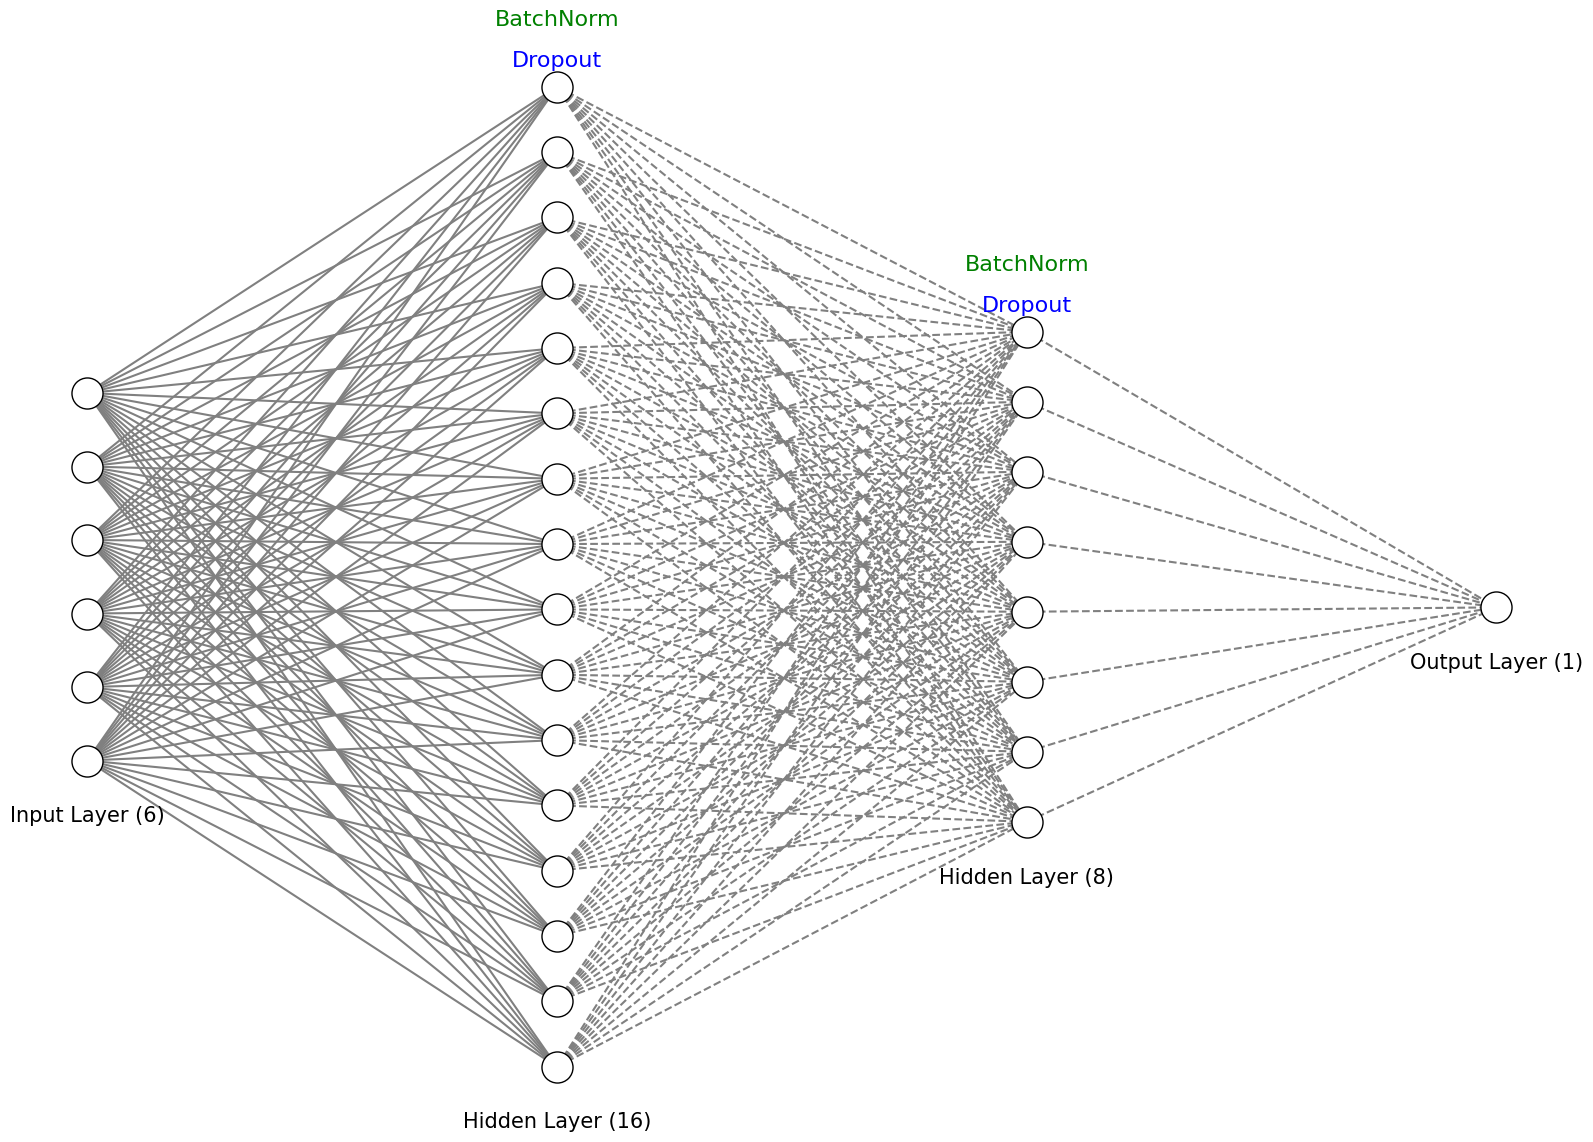
\includegraphics[width=1\textwidth, height=0.7\textheight, keepaspectratio]{ArchitectureOfNN.png}
    \caption{Architecture of our Neural Network, dropout set to 0.2}
\end{figure}



\subsection{Summary}

This methodology provides a simplified yet effective approach to predicting IDT while acknowledging the limitations of the available dataset.We can summarise our methodology by going through the following algorithm

\begin{algorithm}[H]
\SetAlgoLined
\KwResult{Trained models and evaluation metrics}

 \SetKwFunction{FMain}{process}
 \SetKwProg{Fn}{Function}{:}{}
 \Fn{\FMain{df, x\_value, activation, optimizer}}{
    Filter data where \( x \neq \text{x\_value} \)\;
    Select 70\% of data where \( x = \text{x\_value} \)\;
    Concatenate into \texttt{train} dataset and remainder as \texttt{test} dataset\;
    Remove entries where \texttt{idt} is zero in both \texttt{train} and \texttt{test} sets\;
    Apply logarithmic transformation to idt\;
    Define model with batch normalization and dropout\;
    Choose \texttt{optimizer} based on grid search\;
    \texttt{model\_tf.compile(optimizer=optimizer, loss='mse')}\;
    Set callbacks for learning rate scheduling and early stopping\;
    Train model with a larger batch size for better performance\;
    Predict \texttt{idt} values for the \texttt{test} set\;
    Calculate \texttt{MSE}, \texttt{RMSE}, \texttt{R2} and store/plot them\;
 }

 \For{\( \text{x\_value} \) in \texttt{x\_values\_to\_process}}{
    \For{\( \text{activation} \) in \texttt{activation\_functions}}{
        \For{\( \text{optimizer} \) in \texttt{optimizers}}{
            \FMain{df, x\_value, activation, optimizer}\;
        }
    }
 }

 \caption{Data Processing and Model Training Pipeline}
\end{algorithm}


% Content goes here

\chapter{Results and Discussion}
\section{Earlier Results}
Each model was trained on a dataset containing key input features such as equivalence ratio (\(\phi\)), pressure \textit{(p)}, and temperature \textit{(T)}, and was evaluated using standard metrics like mean absolute error (MAE), mean squared error (MSE), and R-squared (\(R^2\)) to assess the model performance.

The selection of these models was made to capture a variety of learning techniques, from instance-based learning with KNN to ensemble methods like Random Forest and Gradient Boosting, and complex neural networks like MLP. Each model’s hyperparameters were carefully tuned to optimize performance and avoid overfitting.

In particular, special attention was given to the trade-off between bias and variance, which plays a crucial role in model selection for combustion-related data. The results presented in the following sections provide insight into each model’s predictive capabilities and potential areas for improvement when applied to the problem of IDT prediction for methane (CH\(_4\)) combustion.

The following sections include the respective plots and an analysis of possible sources of error based on the performance of each model.

\subsection{K-Nearest Neighbors (KNN)}
\textbf{Possible Sources of Errors:} 
\begin{itemize}
    \item KNN is highly sensitive to the choice of the number of neighbors (n\_neighbors). A small value of \(n\) may lead to overfitting as the model becomes too specific to the training data, while a large value could result in underfitting, where important local patterns in the data are smoothed out.
    \item KNN assumes that closer points in the feature space are more relevant, but this assumption may break down when the data contains noise, especially in high-dimensional spaces, leading to poor generalization.
    \item Additionally, KNN does not perform any internal learning; it is computationally expensive during prediction because it must compute distances for every new query, which can introduce inaccuracies if not properly scaled.
\end{itemize}

\subsection{Gradient Boosting}


\textbf{Possible Sources of Errors:} 
\begin{itemize}
    \item Gradient Boosting can be prone to overfitting if the number of estimators (n\_estimators) is too high, particularly if the trees are too deep (max\_depth), leading the model to learn even small, irrelevant fluctuations in the training data.
    \item The learning rate (\( \alpha \)) also plays a critical role. If it is too high, the model may converge too quickly, skipping important patterns, while if it is too low, the model may not converge or may require excessive training time to capture key trends.
    \item Additionally, Gradient Boosting models are sequential, meaning errors propagate from one tree to the next, which could amplify small errors if the earlier trees are not well-tuned.
\end{itemize}

\subsection{Multi-Layer Perceptron (MLP)}


\textbf{Possible Sources of Errors:} 
\begin{itemize}
    \item MLP models are highly sensitive to the choice of hyperparameters like hidden layer sizes and the activation functions. A poorly configured model may take longer to converge or even overfit the training data, especially if the network is too deep.
    \item The solver ('adam') may not perform well on small datasets or may get stuck in local minima during training, leading to suboptimal results.
    \item Furthermore, MLPs can suffer from vanishing or exploding gradient problems depending on the depth of the network and the activation functions chosen. This can prevent proper learning in deep networks, affecting the accuracy of the model.
    \item The complexity of neural networks also means that overfitting is a major concern, especially if not enough regularization techniques, such as dropout or weight decay, are used.
\end{itemize}

\subsection{Decision Tree}

\textbf{Possible Sources of Errors:} 
\begin{itemize}
    \item Decision trees tend to overfit the data if the max\_depth parameter is not carefully controlled. Shallow trees may lead to underfitting, where the model cannot capture complex patterns in the data, while deep trees can become overly sensitive to small variations, resulting in high variance.
    \item Decision trees are particularly prone to instability; small changes in the dataset can lead to very different splits and tree structures, thus making the model less robust to noise or small changes in input data.
    \item Overfitting is also more likely when the tree is allowed to grow fully without pruning or regularization, which can lead to very complex decision boundaries that do not generalize well.
\end{itemize}

\subsection{Random Forest}
\textbf{Possible Sources of Errors:} 
\begin{itemize}
    \item Random Forest models generally reduce overfitting compared to a single decision tree, but they can still suffer from overfitting if the individual trees are too deep or if not enough trees (n\_estimators) are used, which can result in high variance or high bias, respectively.
    \item Furthermore, Random Forest models can become computationally expensive when a large number of trees are built, which can increase training time and memory consumption, especially with large datasets.
    \item Interpretability is also reduced compared to simpler models like decision trees, as it becomes difficult to understand the decision-making process due to the ensemble nature of the model.
\end{itemize}

\subsection{Support Vector Regression (SVR)}
\textbf{Possible Sources of Errors:} 
\begin{itemize}
    \item The choice of the regularization parameter \(C\) and kernel function (in this case, the RBF kernel) has a significant impact on SVR performance. If \(C\) is too high, the model may overfit the data, while if \(C\) is too low, the model may fail to capture the underlying trends, leading to underfitting.
    \item The radial basis function (RBF) kernel may not always be the best choice depending on the distribution of the data. If the data does not exhibit the type of non-linear relationships that RBF excels at capturing, this could result in high bias and poor model performance.
    \item Additionally, SVR can be sensitive to the scaling of the input features. Improperly scaled data can lead to poor convergence and suboptimal performance in higher-dimensional spaces.
\end{itemize}

We can see from the plots pertaining to higher data-points, such as for $\phi$ = 0.5 and \textit{p} = 1 atm, the Gradient Boosting Regressor is able to perform quite well whereas Decision trees and MLP perform quite poorly. As a matter of fact, MLP has performed quite poorly through the entire experiment and this sparks a question about how the other researchers were able to get the best results using ANNs, a cousin of MLP.
\begin{figure}[H]
    \centering
    % First row
    \begin{subfigure}[t]{0.48\textwidth}
        \centering
        \includegraphics[width=\textwidth, keepaspectratio]{Plots_midterm_report/GradientBoostingRegressor_CH4_EqRatio0.5_Pressure1atm_plot.png}
        \caption{Gradient Boosting: \ce{CH4}, $\phi = 0.5$, $p = 1$ atm}
    \end{subfigure}
    \hfill
    \begin{subfigure}[t]{0.48\textwidth}
        \centering
        \includegraphics[width=\textwidth, keepaspectratio]{Plots_midterm_report/GradientBoostingRegressor_CH4_EqRatio0.5_Pressure10atm_plot.png}
        \caption{Gradient Boosting: \ce{CH4}, $\phi = 0.5$, $p = 10$ atm}
    \end{subfigure}

    \vspace{0.5cm} % Add some vertical spacing between rows

    % Second row
    \begin{subfigure}[t]{0.48\textwidth}
        \centering
        \includegraphics[width=\textwidth, keepaspectratio]{Plots_midterm_report/KNeighborsRegressor_CH4_EqRatio0.5_Pressure1atm_plot.png}
        \caption{K Neighbors: \ce{CH4}, $\phi = 0.5$, $p = 1$ atm}
    \end{subfigure}
    \hfill
    \begin{subfigure}[t]{0.48\textwidth}
        \centering
        \includegraphics[width=\textwidth, keepaspectratio]{Plots_midterm_report/KNeighborsRegressor_CH4_EqRatio0.5_Pressure10atm_plot.png}
        \caption{K Neighbors: \ce{CH4}, $\phi = 0.5$, $p = 10$ atm}
    \end{subfigure}

    \caption{Comparisons of Gradient Boosting and K Neighbors models for \ce{CH4} at $\phi = 0.5$ and different pressures.}
\end{figure}

After extensive observation and a new definition of the objective, I concluded that the best model for our use case is the ANN, as it would perform much better with the new methodology devised.



\newpage


\section{Why Neural Networks Now?}
We also found the answer to the question we had asked earlier, why was our ANN not performing as expected? As discussed above, the answer lies in the training dataset itself, we hadn't neglected the 0 entries earlier and so the training dataset was very densely populated with zeroes resulting in the very 'flat' nature of the curves we obtained earlier.

Neural Networks seem to be the appropriate model of choice as when we extend the approach to a more rigorous definiton of the objective that we had layed out i.e varying \textit{p}, $\phi$ and the number of fuels, the ANN architecture could potentially still work, perhaps with more tuning.


\subsection{Summary of Best Configurations}

The table below summarizes the best-performing configurations for each dropout level, activation function, and optimizer combination based on key metrics such as Mean Squared Error (\textbf{MSE}), Root Mean Squared Error (\textbf{RMSE}), validation loss, and \textbf{R²} score.

\begin{table}[h!]
\centering
\caption{Best Configurations for \ce{CH4} fraction, Activation, and Optimizers}
\begin{tabular}{|c|l|l|c|c|c|c|}
\hline
\textbf{\ce{CH4}} & \textbf{Activation} & \textbf{Optimizer} & \textbf{MSE} & \textbf{RMSE} & \textbf{val\_loss} & \textbf{R²} \\ \hline
0       & relu       & SGD       & 0.080952   & 0.284520  & 0.180012    & 0.988472   \\ \hline
0.2     & leaky\_relu & SGD       & 0.066103   & 0.257105  & 0.096906    & 0.992117   \\ \hline
0.4     & elu        & SGD       & 0.060700   & 0.246374  & 0.101666    & 0.993044   \\ \hline
0.8     & selu       & RMSprop   & 0.020965   & 0.144794  & 4.970879    & 0.997478   \\ \hline
0.4     & softplus   & SGD       & 0.031026   & 0.176143  & 0.054062    & 0.996445   \\ \hline
0.6     & swish      & SGD       & 0.029462   & 0.171646  & 0.623092    & 0.996667   \\ \hline
0.8     & gelu       & RMSprop   & 0.084660   & 0.290963  & 3.927773    & 0.989814   \\ \hline
1    & leaky\_relu   & RMSprop   & 0.391455	& 0.625664	& 2.103178	& 0.918333	\\ \hline
\end{tabular}
\label{tab:best_configurations}
\end{table}
\subsection{Sample Plots Obtained}

\begin{figure}[H]
    \centering
    \begin{subfigure}[t]{0.48\textwidth}
        \centering
        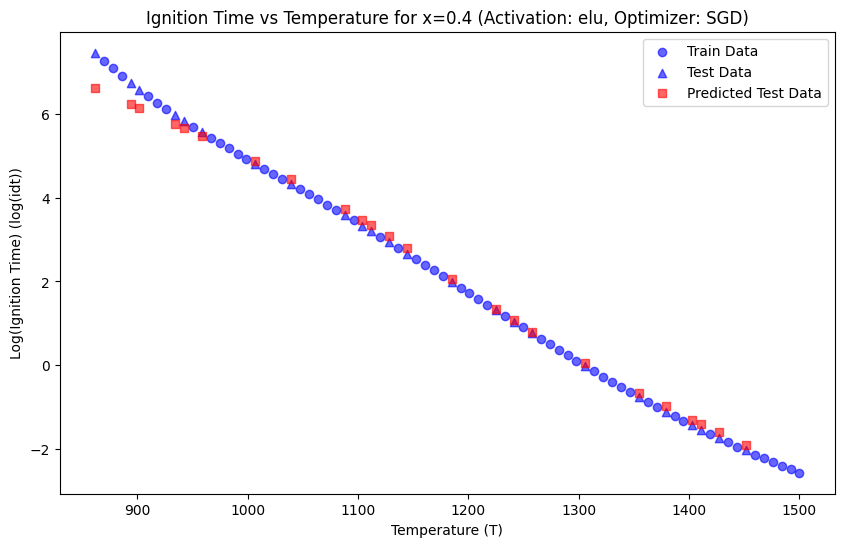
\includegraphics[width=\textwidth, keepaspectratio]{elu_sgd_04.png}
        \caption{ELU with SGD at x=0.2}
    \end{subfigure}
    \hfill
    \begin{subfigure}[t]{0.48\textwidth}
        \centering
        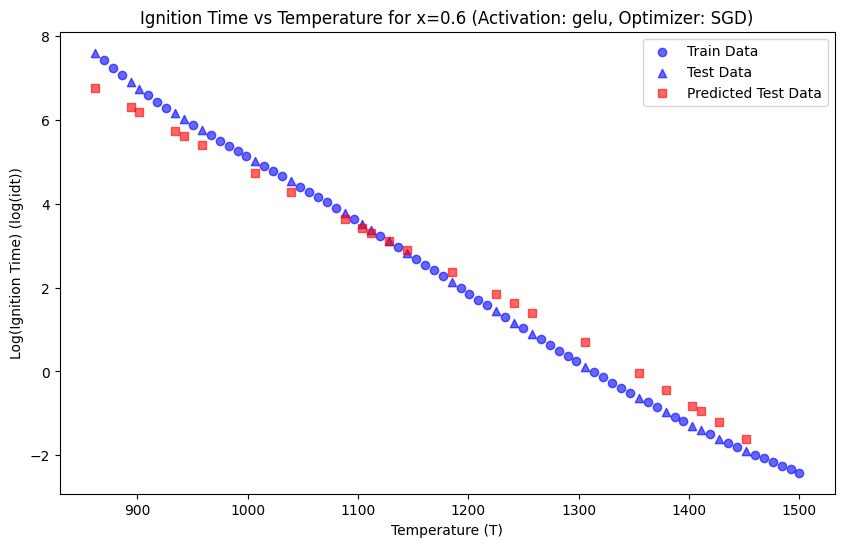
\includegraphics[width=\textwidth, keepaspectratio]{gelu_sgd_06.png}
        \caption{GELU with SGD, x=0.2}
    \end{subfigure}
    % \caption{Comparison of architectures with different configurations (1)}
\end{figure}

\begin{figure}[H]
    \centering
    \begin{subfigure}[t]{0.48\textwidth}
        \centering
        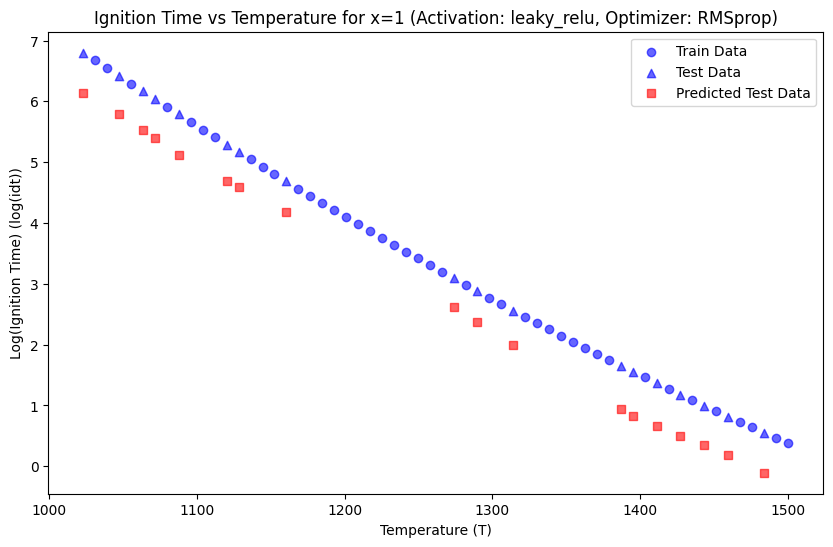
\includegraphics[width=\textwidth, keepaspectratio]{leaky_rms_1.png}
        \caption{Leaky ReLU with RMSProp, x=0.2}
    \end{subfigure}
    \hfill
    \begin{subfigure}[t]{0.48\textwidth}
        \centering
        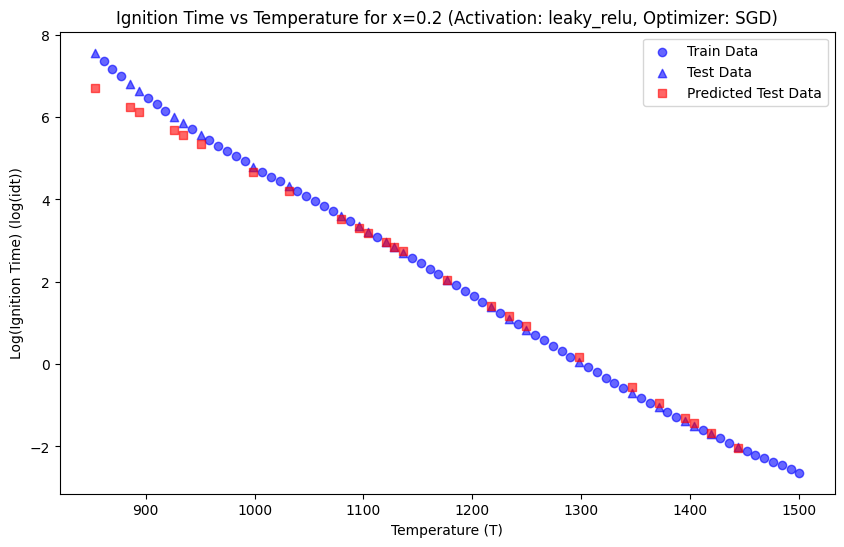
\includegraphics[width=\textwidth, keepaspectratio]{leaky_sgd_02.png}
        \caption{Leaky ReLU with SGD, x=0.2}
    \end{subfigure}
    % \caption{Comparison of architectures with different configurations (2)}
\end{figure}

\begin{figure}[H]
    \centering
    \begin{subfigure}[t]{0.48\textwidth}
        \centering
        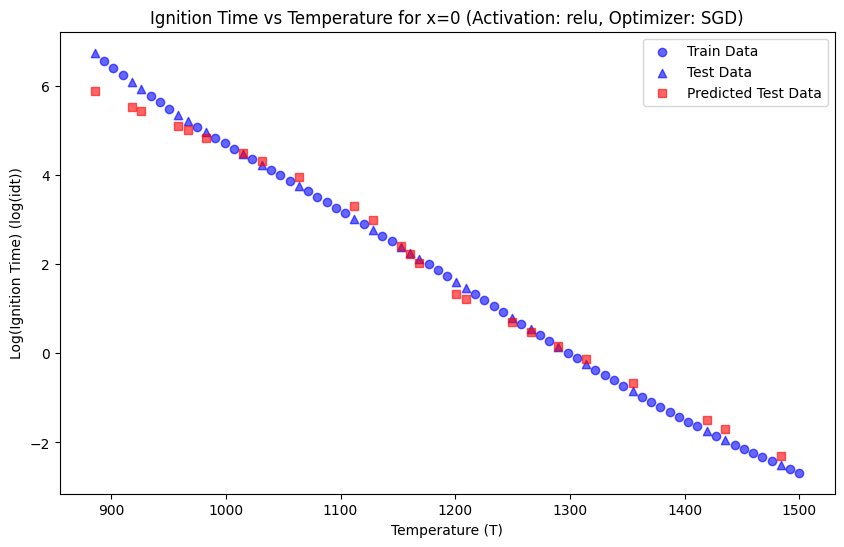
\includegraphics[width=\textwidth, keepaspectratio]{relu_sgd_0.png}
        \caption{ReLU with SGD, x=0.2}
    \end{subfigure}
    \hfill
    \begin{subfigure}[t]{0.48\textwidth}
        \centering
        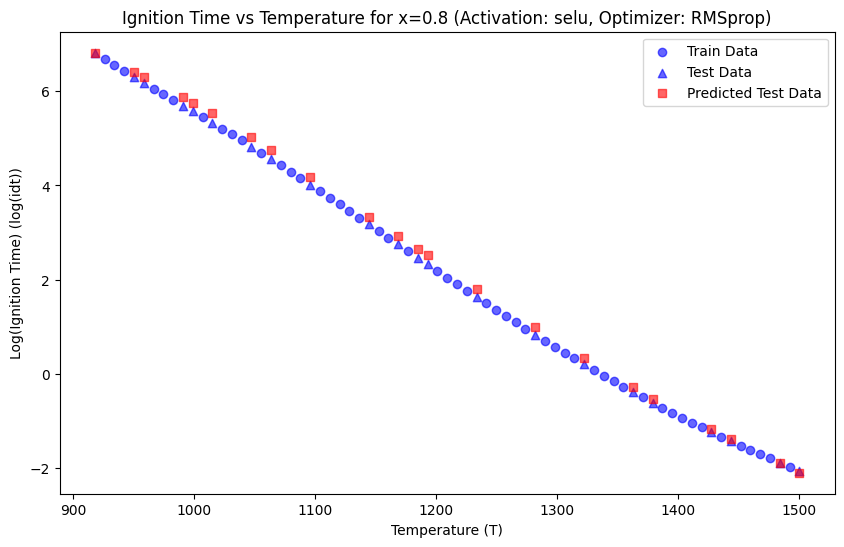
\includegraphics[width=\textwidth, keepaspectratio]{selu_rms_08.png}
        \caption{SELU with RMSProp, x=0.2}
    \end{subfigure}
    % \caption{Comparison of architectures with different configurations (3)}
\end{figure}

\begin{figure}[H]
    \centering
    \begin{subfigure}[t]{0.48\textwidth}
        \centering
        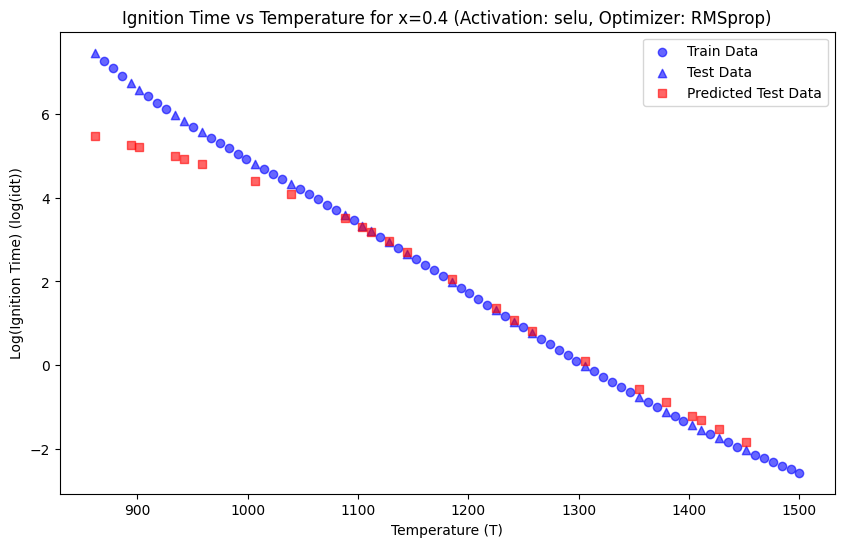
\includegraphics[width=\textwidth, keepaspectratio]{selu_rms_04.png}
        \caption{SELU with RMSProp, x=0.2}
    \end{subfigure}
    \hfill
    \begin{subfigure}[t]{0.48\textwidth}
        \centering
        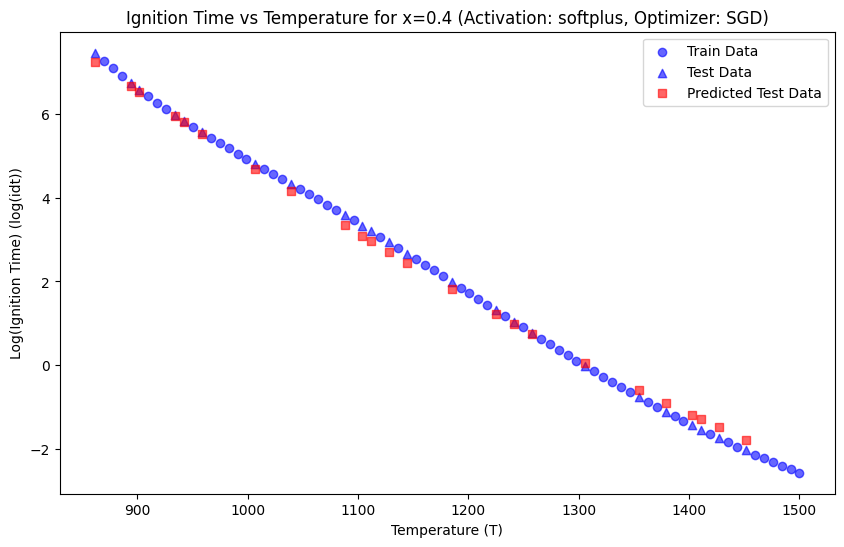
\includegraphics[width=\textwidth, keepaspectratio]{softplus_sgd_04.png}
        \caption{Softplus with SGD, x=0.2}
    \end{subfigure}
    % \caption{Comparison of architectures with different configurations (4)}
\end{figure}

\begin{figure}[H]
    \centering
    \begin{subfigure}[t]{0.48\textwidth}
        \centering
        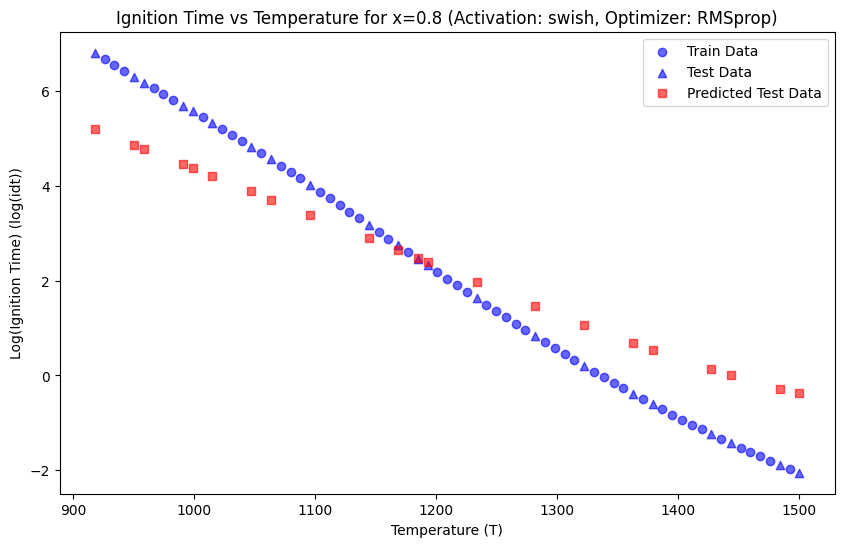
\includegraphics[width=\textwidth, keepaspectratio]{swish_rms_08.png}
        \caption{Swish with RMSProp, x=0.2}
    \end{subfigure}
    \hfill
    \begin{subfigure}[t]{0.48\textwidth}
        \centering
        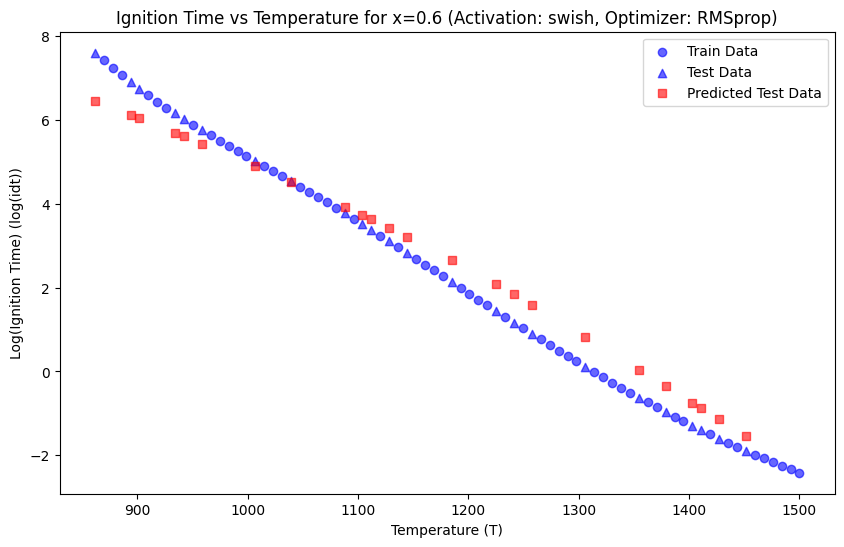
\includegraphics[width=\textwidth, keepaspectratio]{swish_rms_06.png}
        \caption{Swish with RMSProp, x=0.2}
    \end{subfigure}
    % \caption{Comparison of architectures with different configurations (5)}
\end{figure}

\begin{figure}[H]
    \centering
    \begin{subfigure}[t]{0.48\textwidth}
        \centering
        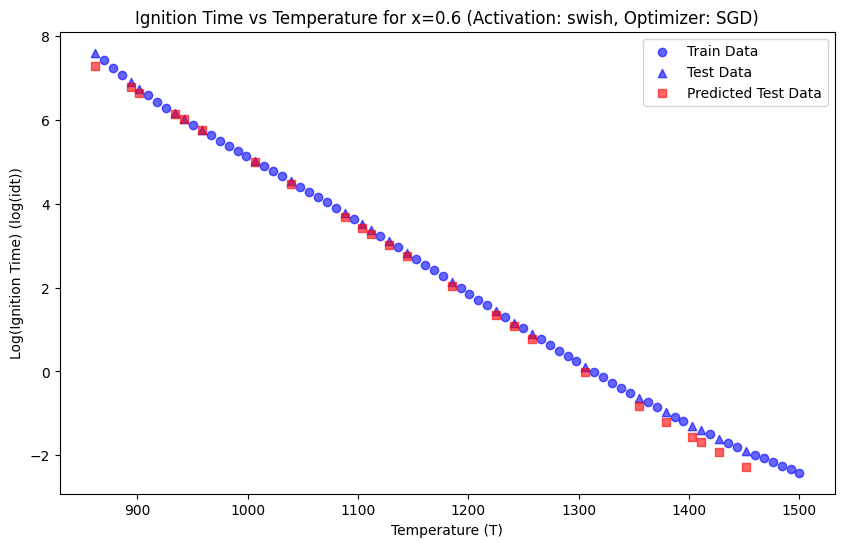
\includegraphics[width=\textwidth, keepaspectratio]{swish_sgd_06.png}
        \caption{Swish with SGD, x=0.2}
    \end{subfigure}
    \hfill
    \begin{subfigure}[t]{0.48\textwidth}
        \centering
        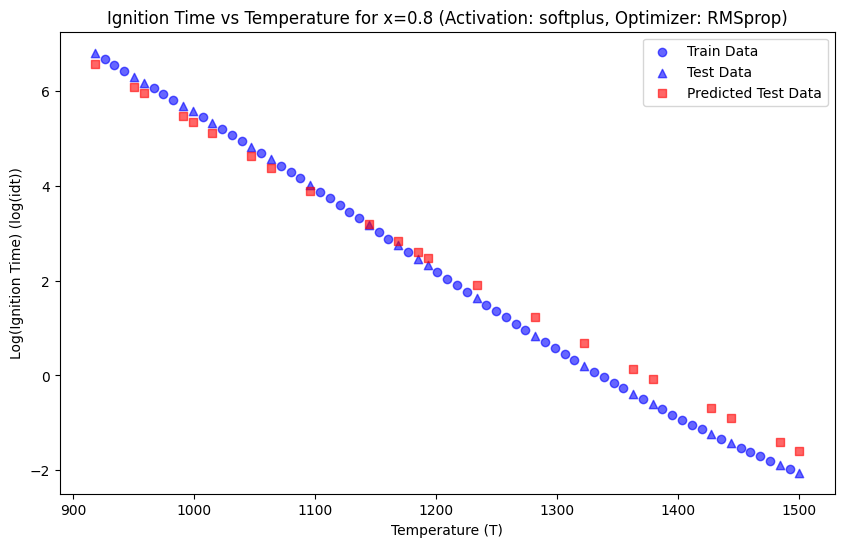
\includegraphics[width=\textwidth, keepaspectratio]{softplus_rms_08.png}
        \caption{Softplus with RMSProp, x=0.2}
    \end{subfigure}
    
    % \caption{Comparison of architectures with different configurations (6)}
\end{figure}




\chapter{Conclusions and Scope of Research}
% Content goes here


\begin{itemize}
    \item \textbf{Hyperparameter Optimization}:
    \begin{itemize}
        \item Optimization was performed on the dropout and number of layers. Using a pseudo-randomized algorithm like simulated annealing for grid search could be useful, though computationally intensive.
    \end{itemize}

    \item \textbf{Expanding the Dataset and Fuel Mixtures}:
    \begin{itemize}
        \item The current model is limited to conditions with \textit{p}=1 atm \& $\phi$=0.5. Expanding the dataset to include a range of pressures and equivalence ratios would broaden the model's applicability.
        \item Thus far, the work has been on \ce{CH4} and \ce{C3H8} mixtures with a small discrete set of \(x\) values. Incorporating fuel mixtures would require the input \( x \) to the neural network would become a set of \( n \) variables.A predefined global set of fuels could allow small modifications to the ANN architecture to handle fractions directly instead of passing them as an \( n \)-dimensional vector.
    \end{itemize}
  

    \item \textbf{Activations and Other Techniques}:
    \begin{itemize}
        \item Developing a custom activation function or optimizer for this specific use-case could be beneficial. 
        \item Investigating different architectures for the ANN, and exploring convolutional neural networks (CNNs) as alternatives, could also be areas for further research.
    \end{itemize}
\end{itemize}



% Nomenclature

\newpage

% References
\begin{thebibliography}{9}

\bibitem{keromnes2013hydrogen}
A. Kéromnès, W. K. Metcalfe, K. A. Heufer, N. Donohoe, A. K. Das, C.-J. Sung, J. Herzler, C. Naumann, P. Griebel, O. Mathieu, M. C. Krejci, E. L. Petersen, W. J. Pitz, and H. J. Curran,
\textit{An experimental and detailed chemical kinetic modeling study of hydrogen and syngas mixture oxidation at elevated pressures}.
Combustion and Flame, 160(6), 995--1011, 2013. DOI: \href{https://doi.org/10.1016/j.combustflame.2013.01.001}{10.1016/j.combustflame.2013.01.001}.

\bibitem{metcalfe2013hierarchical}
W. K. Metcalfe, S. M. Burke, S. S. Ahmed, and H. J. Curran,
\textit{A Hierarchical and Comparative Kinetic Modeling Study of C1--C2 Hydrocarbon Oxidation}.
International Journal of Chemical Kinetics, 45(10), 638--675, 2013. DOI: \href{https://doi.org/10.1002/kin.20802}{10.1002/kin.20802}.

\bibitem{bounaceur2024}
R. Bounaceur, R. Heymes, P.-A. Glaude, B. Sirjean, R. Fournet, P. Montagne, A. Auvray, E. Impellizzeri, P. Biehler, A. Picard, B. Prieur-Garrouste, and M. Molière,
\textit{Development of an Artificial Intelligence Model to Predict Combustion Properties, With a Focus on Auto-Ignition Delay}.
Journal of Engineering for Gas Turbines and Power, 146(6), 061011, 2024. DOI: \href{https://doi.org/10.1115/1.4063774}{10.1115/1.4063774}.

\bibitem{chiesa2005}
P. Chiesa, G. Lozza, and L. Mazzocchi, 
\textit{Using Hydrogen as Gas Turbine Fuel}. 
ASME Journal of Engineering for Gas Turbines and Power, 127(1), 73--80, 2005. DOI: \href{https://doi.org/10.1115/1.1787513}{10.1115/1.1787513}.

\bibitem{burke2016}
U. Burke, W. K. Metcalfe, S. M. Burke, K. A. Heufer, P. Dagaut, and H. J. Curran,
\textit{A Detailed Chemical Kinetic Modeling, Ignition Delay Time and Jet-Stirred Reactor Study of Methanol Oxidation}.
Combustion and Flame, 165, 125--136, 2016. DOI: \href{https://doi.org/10.1016/j.combustflame.2015.11.004}{10.1016/j.combustflame.2015.11.004}.

\bibitem{ignition_model_github}
S. Hegab, 
\textit{Ignition Model}. 
GitHub Repository, 2020. Available: \href{https://github.com/Shimaa/Ignition_Model}{https://github.com/Shimaa/Ignition\_Model}.

\bibitem{rmg_github}
W. H. Green, R. H. West, and contributors, 
\textit{Reaction Mechanism Generator}. 
GitHub Repository, 2020. Available: \href{https://github.com/ReactionMechanismGenerator}{https://github.com/ReactionMechanismGenerator}.

\bibitem{lee1998}
S. Y. Lee and S. Hochgreb,
\textit{Rapid Compression Machine Measurements of Hydrogen Ignition Delays in the Presence of Nitric Oxide}. 
Combustion and Flame, 114(1-2), 531--540, 1998. DOI: \href{https://doi.org/10.1016/S0010-2180(97)00225-7}{10.1016/S0010-2180(97)00225-7}.

\bibitem{mittal2006}
G. Mittal, C.-J. Sung, D. A. Stack, 
\textit{Autoignition of n-Decane Under Low to Moderate Temperature Conditions}. 
Combustion and Flame, 145(1-2), 160--180, 2006. DOI: \href{https://doi.org/10.1016/j.combustflame.2005.09.006}{10.1016/j.combustflame.2005.09.006}.

\bibitem{hong2006}
Z. Hong, D. F. Davidson, R. K. Hanson,
\textit{An Improved H2/O2 Mechanism Based on Recent Shock Tube/laser Absorption Measurements}. 
Combustion and Flame, 144(1-2), 25--36, 2006. DOI: \href{https://doi.org/10.1016/j.combustflame.2005.06.005}{10.1016/j.combustflame.2005.06.005}.

\bibitem{troe2011}
J. Troe,
\textit{Combustion Reactions of the Hydrogen Molecule in High-Pressure Situations}. 
Journal of Physical Chemistry, 115(31), 8675--8683, 2011. DOI: \href{https://doi.org/10.1021/jp201474r}{10.1021/jp201474r}.

\bibitem{walton2007}
S. M. Walton, J. M. Deveau, R. S. Tranter, 
\textit{Pressure and Temperature Dependence of Hydrogen Combustion in the Presence of CO2}. 
Journal of Physical Chemistry A, 111(36), 8463--8470, 2007. DOI: \href{https://doi.org/10.1021/jp072183j}{10.1021/jp072183j}.

\bibitem{you2011}
X. You, Z. Wang, C. Sung,
\textit{On the Oxidation Kinetics of Hydrogen and Syngas: Modeling and Experimental Investigations}. 
International Journal of Hydrogen Energy, 36(8), 4566--4579, 2011. DOI: \href{https://doi.org/10.1016/j.ijhydene.2011.01.132}{10.1016/j.ijhydene.2011.01.132}.

\bibitem{zhao2008}
R. Zhao, D. Xie, J. Cai,
\textit{Experimental Study on the Combustion Characteristics of Syngas in a High-Pressure Environment}. 
Energy & Fuels, 22(3), 1807--1812, 2008. DOI: \href{https://doi.org/10.1021/ef700709f}{10.1021/ef700709f}.

\bibitem{bradley2005}
D. Bradley, M. S. Harper, and M. Lawes,
\textit{The Measurement of Laminar Burning Velocities and Markstein Numbers for Iso-octane–air and iso-octane–n-heptane–air Mixtures at Elevated Temperatures and Pressures in an Explosion Bomb}. 
Combustion and Flame, 138(1-2), 55--71, 2004. DOI: \href{https://doi.org/10.1016/j.combustflame.2004.04.002}{10.1016/j.combustflame.2004.04.002}.

\bibitem{burke2010}
M. P. Burke, M. Chaos, Y. Ju, F. L. Dryer,
\textit{Comprehensive Modeling Study of Hydrogen and Syngas Combustion with Comparison to Experimental Data}. 
International Journal of Chemical Kinetics, 42(4), 198--231, 2010. DOI: \href{https://doi.org/10.1002/kin.20482}{10.1002/kin.20482}.

\bibitem{petersen2008}
E. Petersen, M. Hall, H. Smith, B. C. Conley, 
\textit{Ignition Delay Times for Methane and Ethane in Shock Tubes at Elevated Pressures: Computational Chemistry for Engine Simulations}. 
Combustion and Flame, 152(3), 294--296, 2008. DOI: \href{https://doi.org/10.1016/j.combustflame.2007.10.006}{10.1016/j.combustflame.2007.10.006}.

\bibitem{krejci2011}
M. C. Krejci, E. L. Petersen, W. P. Klingshirn, 
\textit{Experimental Investigation of the Autoignition Characteristics of Ethanol/Gasoline Blends}. 
Fuel, 90(2), 623--634, 2011. DOI: \href{https://doi.org/10.1016/j.fuel.2010.09.040}{10.1016/j.fuel.2010.09.040}.

\bibitem{veloo2011}
P. S. Veloo and F. L. Dryer, 
\textit{Direct Experimental Study of Laminar Flowing Methanol–air Flame Structure and Modeling Comparison}. 
Combustion and Flame, 158(1), 67--72, 2011. DOI: \href{https://doi.org/10.1016/j.combustflame.2010.06.016}{10.1016/j.combustflame.2010.06.016}.

\bibitem{vancoillie2013}
J. Vancoillie, L. Sileghem, S. Verhelst, 
\textit{Comparison of the Alternative Fuels Methanol, Ethanol and Methane for Passenger Cars in Relation to Energy Efficiency and CO$_2$ Emissions}. 
Energy Policy, 48, 594--601, 2013. DOI: \href{https://doi.org/10.1016/j.enpol.2012.05.052}{10.1016/j.enpol.2012.05.052}.

\bibitem{shaoanlu2017} 
S. Lu, 
\textit{SGD \& All: Which One Is the Best Optimizer? Dogs vs. Cats Toy Experiment}. 
May 2017. [Online]. Available: \href{https://shaoanlu.wordpress.com/2017/05/29/sgd-all-which-one-is-the-best-optimizer-dogs-vs-cats-toy-experiment/}{shaoanlu.wordpress.com}.

\bibitem{reddi2017}
S. J. Reddi, S. Kale, S. Kumar,
\textit{On the Convergence of Adam and Beyond}. 
arXiv preprint, 2017. DOI: \href{https://arxiv.org/abs/1705.08292}{10.48550/arXiv.1705.08292}.

\bibitem{shaoanluGithub2017}
S. Lu, 
\textit{Dogs vs. Cats Redux: Optimizer Experiment Notebook}, 
GitHub Repository, May 2017. [Online]. Available: \href{https://github.com/shaoanlu/dogs-vs-cats-redux/blob/master/opt_experiment.ipynb}{github.com}.

\bibitem{stackexchange2018}
\textit{Why Not Always Use the Adam Optimization Technique?}, 
Data Science Stack Exchange, 2018. [Online]. Available: \href{https://datascience.stackexchange.com/questions/30344/why-not-always-use-the-adam-optimization-technique}{datascience.stackexchange.com}.
 

\end{thebibliography}








\end{document}
